\setlength{\columnsep}{3pt}
\begin{flushleft}

\begin{itemize}
	\item Download VirtualBox hypervisior from \textbf{https://www.virtualbox.org/wiki/Downloads} 
	according to your OS:
	\begin{figure}[h!]
		\centering
		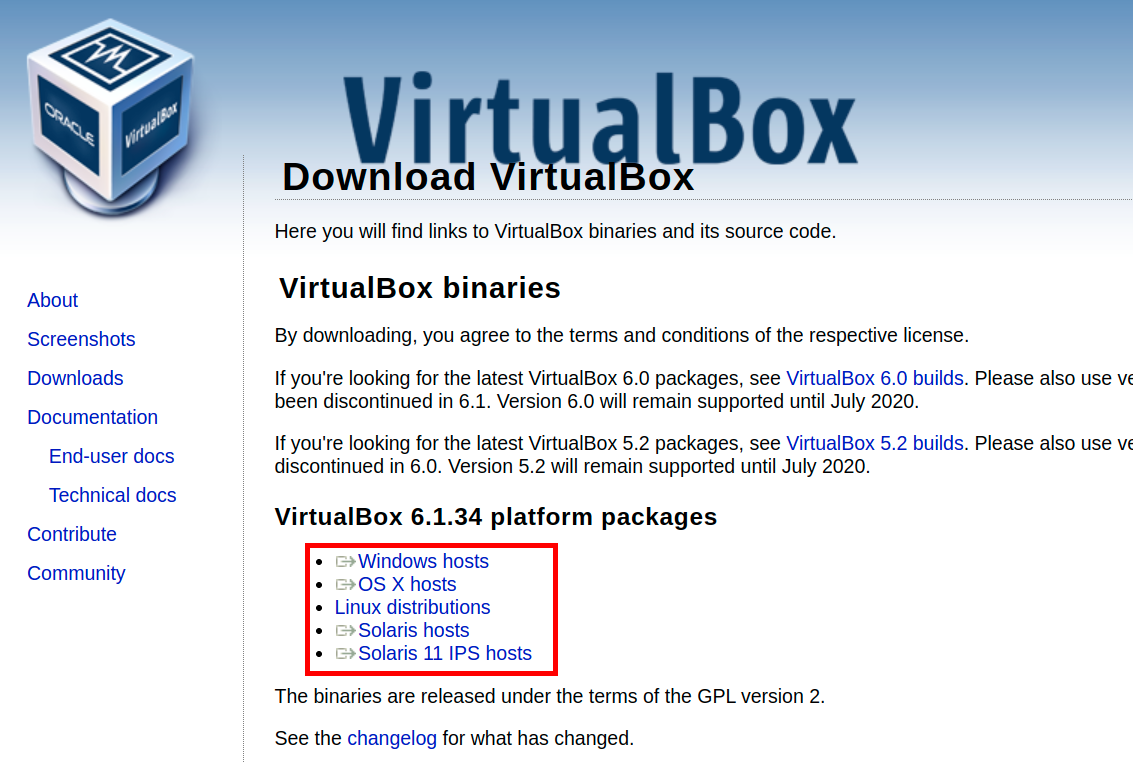
\includegraphics[scale=.25]{content/chapter18/images/vm.png}
	\end{figure}		

	\item Install VirtualBox by running the executable file.	
	
	\item Next, download RHEL8 ISO from \textbf{https://developers.redhat.com/products/rhel/download}
	
	\begin{figure}[h!]
		\centering
		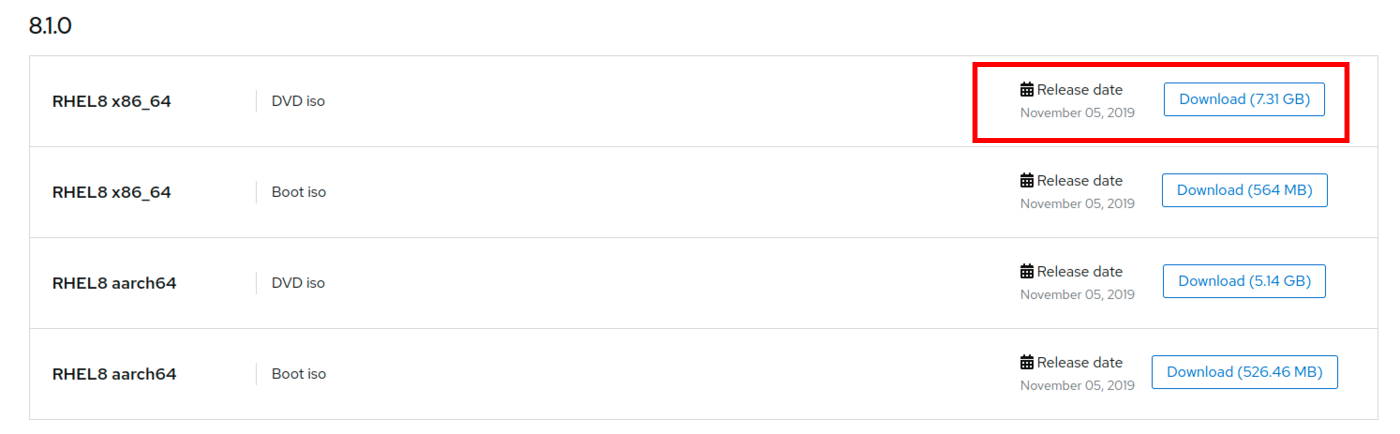
\includegraphics[scale=.2]{content/chapter18/images/iso.png}
		\caption{Download ISO by clicking on red box}
		\label{new}
	\end{figure}		

	\newpage
	\item Open the VirtualBox application and create a new virtual machine(VM) by clicking on new button:
	
	\begin{figure}[h!]
		\centering
		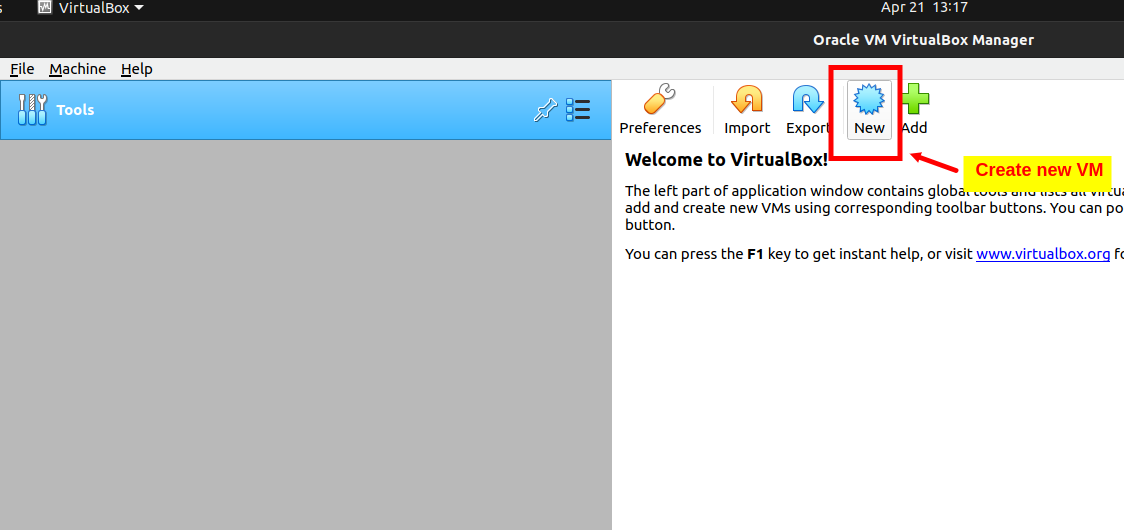
\includegraphics[scale=.23]{content/chapter18/images/image1.png}
	\end{figure}		

	\item Provide name to the VM and click next.
	\begin{figure}[h!]
		\centering
		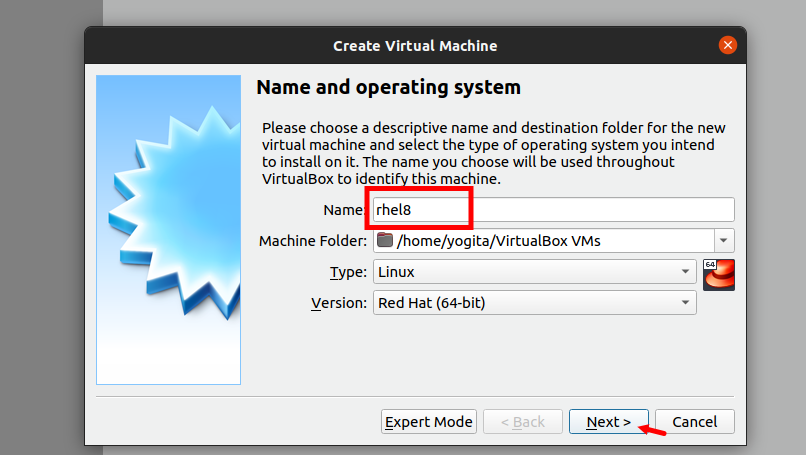
\includegraphics[scale=.3]{content/chapter18/images/image2.png}
	\end{figure}		
	
	\item Enter the RAM size for the VM.
	\begin{figure}[h!]
		\centering
		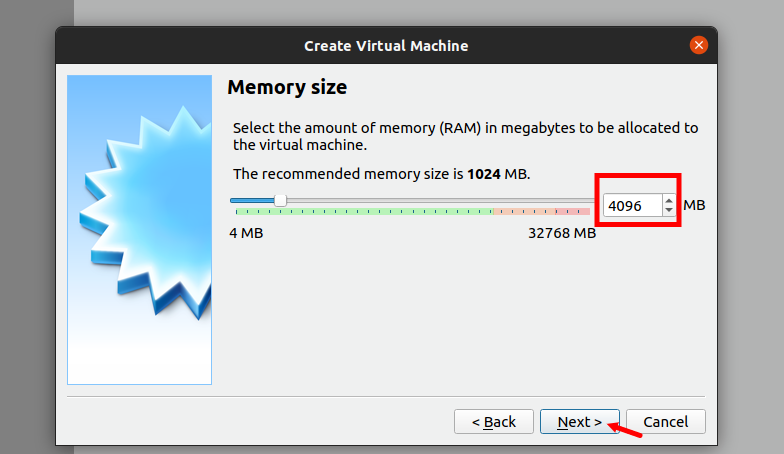
\includegraphics[scale=.3]{content/chapter18/images/image3.png}
	\end{figure}		

	\newpage
	\item Create a virtual HDD as shown.
	\begin{figure}[h!]
		\centering
		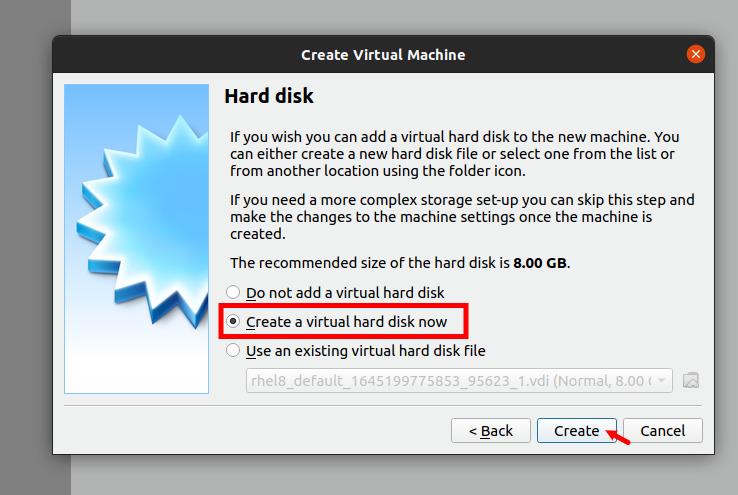
\includegraphics[scale=.3]{content/chapter18/images/image4.png}
	\end{figure}		

	
	\item Select HDD file type as VDI as shown in the image:
	\begin{figure}[h!]
		\centering
		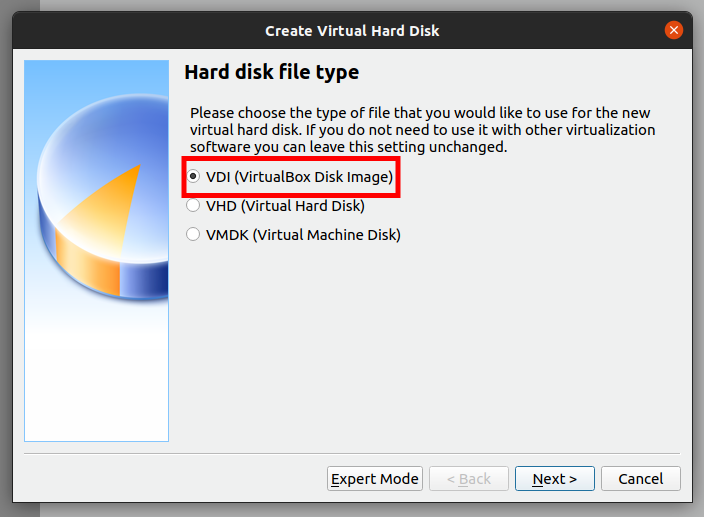
\includegraphics[scale=.3]{content/chapter18/images/image5.png}
	\end{figure}		
	
	\item Select the \textbf{"Dynamically allocated"} option so that VM will use physical HDD space as it fills up.
	
	\begin{figure}[h!]
		\centering
		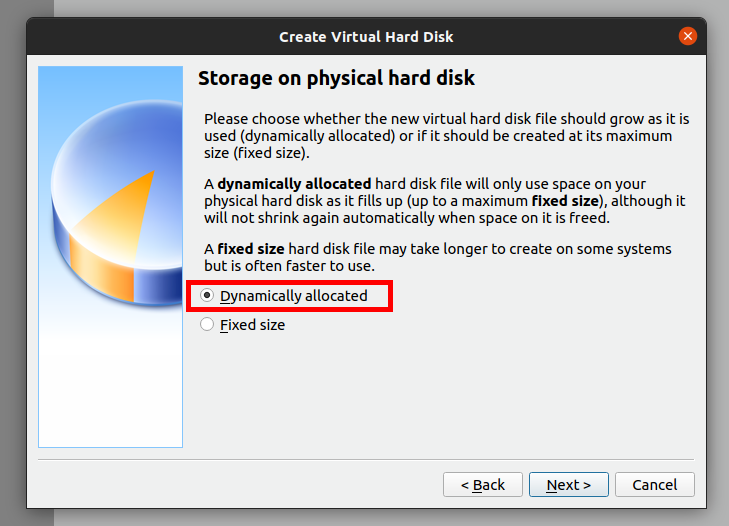
\includegraphics[scale=.25]{content/chapter18/images/image6.png}
	\end{figure}		
	
	\newpage
	
	\item Enter the virtual HDD size for the VM as per your requirement. In the screenshot shown, the HDD size entered is 20GB.
	
	\begin{figure}[h!]
		\centering
		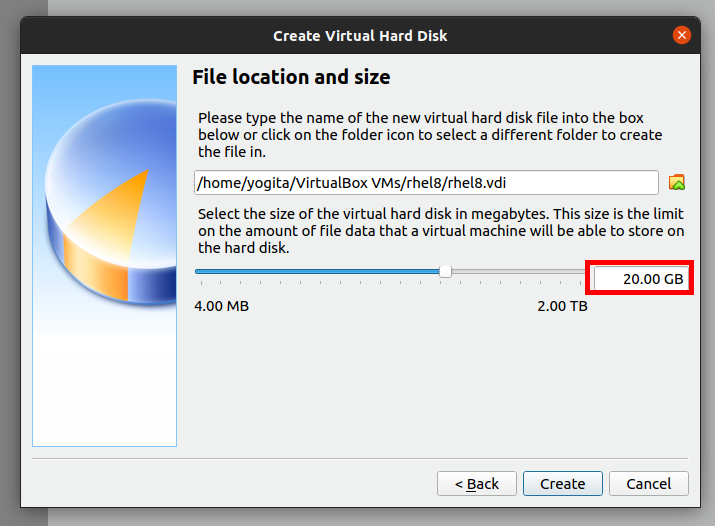
\includegraphics[scale=.25]{content/chapter18/images/image7.png}
	\end{figure}		
	
	\item Now select \textbf{"Storage"} option to upload RHEL8 ISO.
	\begin{figure}[h!]
		\centering
		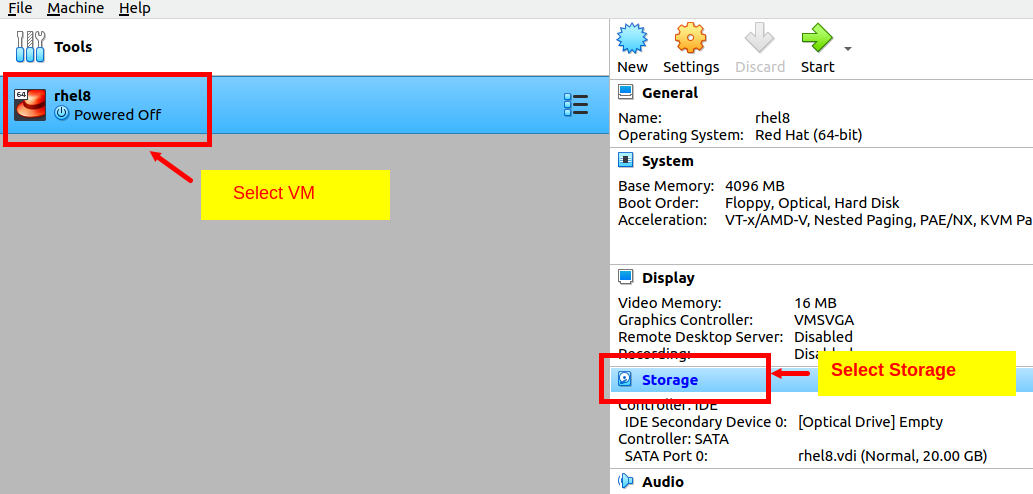
\includegraphics[scale=.25]{content/chapter18/images/image8.png}
	\end{figure}		
	

	\item Upload RHEL 8 ISO by selecting the drive icon as shown.
	\begin{figure}[h!]
		\centering
		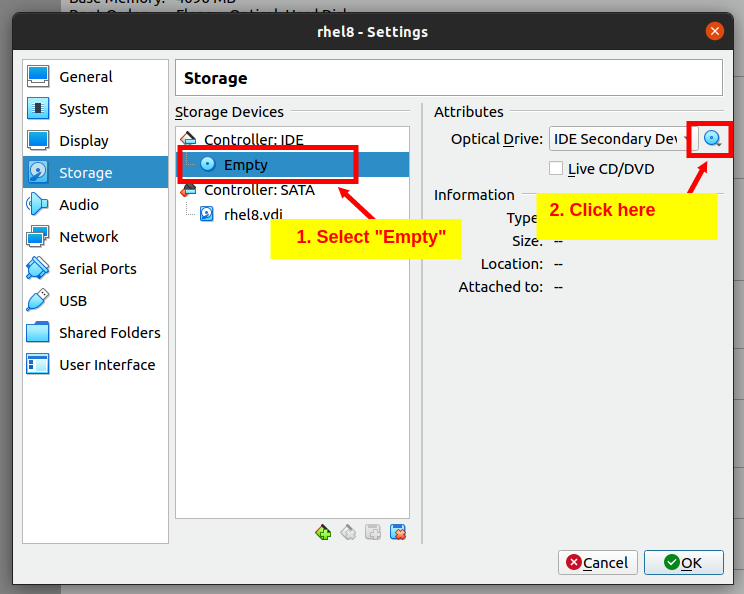
\includegraphics[scale=.3]{content/chapter18/images/image9.png}
	\end{figure}		
	
	\newpage
	This is how the uploaded ISO should look like:
	\begin{figure}[h!]
		\centering
		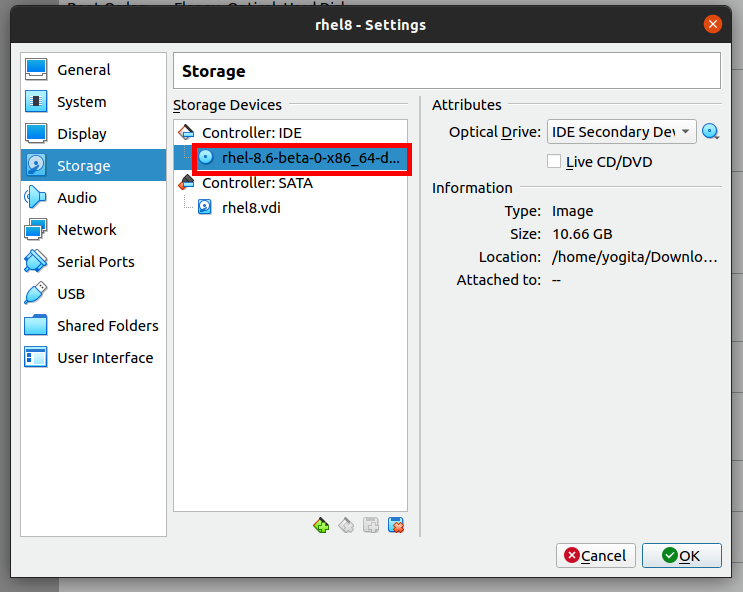
\includegraphics[scale=.3]{content/chapter18/images/image10.png}
	\end{figure}		
	
\end{itemize} 
 
\end{flushleft}
\newpage


